\documentclass[
  aps,
  reprint,
  superscriptaddress,
  floatfix,
  nofootinbib,
  longbibliography
]{revtex4-2}

\usepackage{amsmath,amssymb}
\usepackage{graphicx}
\usepackage{xcolor}
\usepackage{tikz}
\usetikzlibrary{calc,positioning,arrows.meta}
\usepackage{hyperref}

\hypersetup{
  colorlinks=true,
  linkcolor=blue,
  citecolor=blue,
  urlcolor=blue
}

% --- convenience macros -------------------------------------------------
\newcommand{\R}{\mathbb{R}}
\newcommand{\E}{\mathbb{E}}
\newcommand{\Prob}{\mathbb{P}}
\newcommand{\Sph}[1]{S^{#1}}
\newcommand{\Nsem}{N}
\newcommand{\sint}{\sigma_{\mathrm{int}}}
\newcommand{\Eint}{E_{\mathrm{int}}}
\newcommand{\T}{^{\mathsf{T}}}
\newcommand{\opnorm}[1]{\lVert #1 \rVert_{\mathrm{op}}}
\newcommand{\norm}[1]{\lVert #1 \rVert}
\newcommand{\ReLU}{\mathrm{ReLU}}

\DeclareMathOperator*{\argmax}{arg\,max}
\DeclareMathOperator{\spanop}{span}
\DeclareMathOperator{\Var}{Var}

\begin{document}

\title{Geometric Limits on Semantic Expressibility: Quantum-Inspired Contexts and Polysemy in Large Language Models}

\author{Karl Svozil}
\email{karl.svozil@tuwien.ac.at}
\affiliation{Institute for Theoretical Physics, TU Wien,
Wiedner Hauptstra\ss{}e 8--10/136, 1040 Vienna, Austria}

\date{\today}

\begin{abstract}
A fixed-width language-model representation may encode a semantic feature
dictionary larger than its usable carrier dimension while exposing only a
context-dependent subset at any one time.  Let $d$ denote the dimension of a
declared usable carrier and let $\Nsem$ denote the number of feature directions
obtained by a prespecified extraction rule.  We study the overcomplete regime
$\Nsem>d$ as a modelling premise, not as a capacity result.  For an isotropic
random dictionary, extreme-value concentration predicts
\[
 \mu_{\max}^{\rm null}
 \approx 2\sqrt{\frac{\log \Nsem}{d}},
\]
so a chosen overlap tolerance $\varepsilon$ defines the crowding scale
$N_{\rm crowd}(d,\varepsilon)\approx\exp(d\varepsilon^2/4)$.  This is a
calibrated null prediction, not a hard upper bound on learned or optimized
codes.  Simultaneous linear readout imposes a different constraint: for $k$
random-like active directions, interference scales as $\sqrt{k/d}$.  The
sharper semantic prediction is that learning allocates smaller overlaps to
features that frequently coactivate, thereby reducing coactivation-weighted
interference relative to isotropic and activity-matched controls.

On this classical baseline we formulate a separate, stronger model of
polysemy.  Context observables share a token-associated spectral projector but
act differently, and potentially noncommutatively, on sense subspaces in its
orthogonal complement.  Conditional projection then produces a contextual
embedding.  The model is quantum-inspired rather than physically quantum, and
its scientific content is the testable claim that the shared-projector
structure improves held-out prediction, compression, or order-sensitive
contextual readout relative to parameter-matched classical alternatives.
\end{abstract}

\maketitle


% ======================================================================
\section{Introduction}
\label{sec:intro}
% ======================================================================

This chapter examines contextual representation in large language models
(LLMs) as part of the volume's broader inquiry into ``quantum thinking.''
Only a minimal orientation to LLM operation is needed here.  Input text is
first divided into tokens, and each token is mapped to an initial vector.
Transformer blocks then use self-attention and feed-forward transformations
to turn those initially context-free vectors into sequence-dependent hidden
states~\cite{Vaswani-2017-Attention}.  An output layer converts the final state into token scores, and a
softmax distribution supports probabilistic next-token selection.  This
compact chain---tokens, embeddings, contextual transformation, and finite
readout---supplies the computational background for the argument below; the
details of pre-training, fine-tuning, reinforcement learning, and
backpropagation are not required.

Current Transformer-based LLMs are classical computational systems.  They
run on classical hardware and use real-valued matrix operations,
normalization, nonlinearities, copying, and generally irreversible updates.
Their reliance on vectors, inner products, high dimension, or probabilistic
output does not by itself make them quantum or even quantum-like.  The more
limited question pursued here is where ordinary high-dimensional geometry
already explains the coexistence and contextual selection of semantic
features, and where a stronger comparison with quantum-like formalisms might
begin.  Such a comparison would have to do more than rename familiar neural
operations: it would need to identify a role for contextual bases or subspaces,
incompatible or noncommuting alternatives, interference, or
measurement-like readout that yields explanatory or predictive value beyond
a classical dynamic-embedding account.

Semantic concurrency makes this boundary concrete.  A model must preserve
many latent possibilities while making only a small, context-selected subset
operationally accessible.  Polysemy is the simplest illustration: the same
token can participate in financial, river-edge, or seat/bench contexts of
``bank,'' yet the surrounding sequence drives it toward different contextual
representations.  Here polysemy concerns related senses and is distinguished
from homonymy~\cite{pustejovsky1995}.  The verb in an aircraft ``banks'' supplies a fourth sense,
mentioned below but not used in the three-arm schematic.  This relation among
possibility, context, and readout
connects directly to the volume's recurring themes without implying that the
underlying machine is physically quantum.  It also motivates a separation
between what a representation can geometrically accommodate and what a
finite channel can reliably recover.



The claims below occupy different rungs of that evidential ladder.  Frame
coherence, spherical concentration, and correlation-readout estimates are
standard mathematics; here they serve only as calibrated classical nulls
subject to stated assumptions about the usable carrier, feature extractor,
metric, and coactivation.  The reference-subspace organization is
a stronger empirical hypothesis about LLM internals and is tested against
classical controls.  The comparison with quantum contextuality remains a
limited structural correspondence; no physical quantumness, Born-rule
dynamics, or semantic Kochen--Specker theorem is inferred.

The geometric question begins only after an overcomplete semantic dictionary
has been operationally identified.  Let $d$ be the dimension of the usable
carrier after a declared restriction or whitening procedure, and let $\Nsem$
be the number of distinct feature directions returned by a prespecified
dictionary-extraction and duplicate-removal rule.  We study the case
$\Nsem>d$.  This inequality merely specifies the domain in which exact mutual
orthogonality is impossible; it is not itself a finding, and no semantic
deficiency is attributed to representations with $\Nsem\leq d$.

The first substantive question is quantitative: at fixed $d$ and $\Nsem$,
how much interference should an unstructured overcomplete code produce, and
does training reorganize that interference in a semantically useful way?  For
an isotropic random dictionary, the largest of order $\Nsem^2$ pairwise
overlaps is expected to scale as
%
\begin{equation}
\label{eq:intro-capacity}
\mu_{\max}^{\rm null}
\approx 2\sqrt{\frac{\log\Nsem}{d}}.
\end{equation}
%
Equivalently, a prescribed tolerance $\varepsilon$ defines the random-code
crowding scale
$N_{\rm crowd}(d,\varepsilon)\approx\exp(d\varepsilon^2/4)$.  This is a null
benchmark, not a hard limit on spherical codes or learned representations.

Worst-pair overlap alone is not a semantic criterion.  Two features that are
never jointly required may overlap without impairing readout, whereas a much
smaller overlap between frequently coactive features can be costly.  If $k$
random-like directions are active with order-one amplitudes, the baseline
linear-readout interference is
%
\begin{equation}
\label{eq:intro-readout}
\sint\sim\sqrt{\frac{k}{d}}.
\end{equation}
%
The sharper prediction developed below weights squared overlaps by empirical
coactivation.  At matched $d$, $\Nsem$, activity, and feature importance, a
semantically organized dictionary should reduce this weighted interference
relative to isotropic and suitably matched controls.  That comparison, rather
than the elementary inequality $\Nsem>d$, supplies a falsifiable geometric
claim.

The chapter therefore advances two independent hypotheses.  The first is that
learned feature geometry can be evaluated against explicit random-code and
coactivation-aware interference baselines.  The second concerns the internal
organization of polysemy: for some canonically polysemous tokens, context may
be represented by symmetric operators that share a stable token-associated
spectral projector while differing on low-dimensional sense subspaces in its
orthogonal complement.  These operators may fail to commute, and their
conditional projections define contextual embeddings.  Concentration
geometry does not imply this operator structure; it earns scientific content
only if it improves held-out prediction or compression over dimension- and
parameter-matched unstructured models.  Section~\ref{sec:predictions} states
how both hypotheses can fail.

A serious caveat is anisotropy.  The nominal width of an LLM layer may exceed
the dimension of the carrier actually occupied by its states.  To avoid a
third dimensional symbol, $d$ throughout this chapter means the \emph{usable
exact dimension}: first restrict or whiten the representation to the carrier
being tested, then let $d$ be the size of an orthonormal basis of that carrier.
If this usable $d$ is small, the random-code crowding and readout baselines
worsen.  The
method used to identify the carrier must therefore be declared empirically.

The reference-subspace and operator hypotheses have a narrower domain. They
are meant for
canonically polysemous tokens with established sense inventories, such
as WordNet-, OntoNotes-, SemCor-, or WiC-style sense
distinctions~\cite{pilehvar2019wic} with enough contextual instances
for testing. Failure on a representative sample, against the controls in
Sec.~\ref{sec:predictions}, would count against a privileged token reference
subspace or shared-sector operator model even if the broader null calibration
survives.

The proposal is adjacent to the superposition hypothesis in mechanistic
interpretability~\cite{elhage2022superposition}, according to which neural networks
represent more features than they have neurons by packing features into
nearly orthogonal directions. The present chapter separates the
geometric background from a possible semantic organization within it.
The general superposition picture concerns an overcomplete dictionary
of feature directions and sparse active sets. The present model adds the more
specific possibility that contextual readout is organized around stable
token-associated directions and context-dependent, potentially noncommuting
projectors.

Section~\ref{sec:concentration} develops the geometric null model:
the deterministic coherence floor, an isotropic random-dictionary baseline,
and the distinction between dictionary coexistence and simultaneous readout,
culminating in the task-dependent criterion of
Sec.~\ref{sec:operating-criterion}. Section~\ref{sec:reference} introduces the
reference-subspace hypothesis, its shared-sector projector and observable
parameterization, and its relation to dynamic contextual embeddings.
Section~\ref{sec:attention} connects the construction to attention as soft
context routing rather than literal basis reconstruction.
Section~\ref{sec:discussion} discusses superposition, sparse
autoencoders, limitations, empirical tests, and the limited quantum
analogy.

{Global variables and local ranks.}
Throughout, $\R^{d}$ is the usable Euclidean carrier, and $d$ is its exact
integer dimension.  The symbol $\Nsem$ is the size of a prespecified semantic
feature dictionary; it is a count of directions, not another dimension.  A
dictionary is called overcomplete when $\Nsem>d$, and its directions are
called $\varepsilon$-quasi-orthogonal only if their measured overlaps satisfy
the criterion below.  The symbol $k$ counts the directions active in one
context.  The quantities $\varepsilon$ and the later decision margin $\Delta$
are tolerances, while $p$ and $q_C$ are local ranks of particular reference
and sense subspaces.  None is a second global vector-space dimension.

The carrier has inner product $u\T v$
and norm $\norm{v}=\sqrt{v\T v}$; $\Sph{d-1}=\{v\in\R^{d}:\norm{v}=1\}$
is the unit sphere; $I$ is the identity matrix; $\opnorm{\cdot}$ is the
operator norm; $A\succeq0$ means positive semidefinite; and $\Prob$ and
$\E$ denote probability and expectation under the uniform measure on
the relevant sphere unless stated otherwise. Universal positive
constants are denoted $c,c'$, possibly changing from line to line.

% ======================================================================
\section{A geometric null model for an overcomplete dictionary}
\label{sec:concentration}
% ======================================================================

The results recalled in this section are standard facts about frames,
spherical concentration, and correlation readout.  No new packing theorem is
claimed.  Their role is to define a quantitative null model against which an
empirically extracted feature dictionary can be compared.  The quantities
$d$, $\Nsem$, the metric, the extraction rule, and the readout must therefore
be fixed before the comparison is made.

\subsection{Overcomplete dictionaries and a hard coherence floor}
\label{sec:quasiortho}

Let $w_1,\dots,w_{\Nsem}\in\R^d$ be unit feature directions obtained by a
prespecified procedure, and assume throughout this section that $\Nsem>d$.
This is the domain under study, not a conclusion about semantic usefulness.
The mutual coherence is
%
\begin{equation}
\label{eq:quasiortho}
\mu(W)=\max_{i\ne j}|w_i\T w_j|.
\end{equation}
%
We call the dictionary $\varepsilon$-quasi-orthogonal when
$\mu(W)\le\varepsilon$.  The term ``pseudo-orthogonal'' is avoided because it
normally refers to an indefinite inner-product geometry.

Unlike the elementary observation that an overcomplete family cannot be
mutually orthogonal, the Welch bound supplies a quantitative, deterministic
coherence floor:
%
\begin{equation}
\label{eq:welch}
\mu(W)^2\ge
\frac{\Nsem-d}{d(\Nsem-1)}
\qquad (\Nsem>d)
\end{equation}
%
for every unit-vector dictionary~\cite{welch1974coherence}.  This is a genuine
geometric constraint, but it is often too weak to predict the largest overlap
of a particular learned dictionary.  For that purpose we next introduce an
isotropic random baseline.

\subsection{Isotropic random-dictionary baseline}
\label{sec:levy}

For independent uniform unit vectors $u,v\in\Sph{d-1}$,
%
\begin{equation}
\label{eq:moments}
\E[u\T v]=0,
\qquad
\Var(u\T v)=\frac{1}{d},
\end{equation}
%
and spherical concentration gives, up to an inessential choice of constants,
%
\begin{equation}
\label{eq:overlap}
\Prob\{|u\T v|\ge\varepsilon\}
\le 2\exp\!\left[-\frac{(d-1)\varepsilon^2}{2}\right]
\end{equation}
%
for the small-overlap regime of interest~\cite{ledoux2001concentration,milman1986asymptotic}.
A union bound for $\Nsem$ independently sampled directions yields
%
\begin{equation}
\label{eq:unionbound}
\Prob\{\mu(W)\ge\varepsilon\}
\lesssim
\Nsem^2\exp(-c d\varepsilon^2).
\end{equation}
%
Equation~\eqref{eq:unionbound} is a sufficient high-probability statement for
a random construction.  It is not an upper bound on optimized spherical codes
and is not a semantic impossibility theorem.

Ignoring polynomial prefactors in the spherical-cap tail, the typical largest
overlap in the random ensemble satisfies
%
\begin{equation}
\label{eq:max-overlap}
\mu_{\max}^{\rm null}(d,\Nsem)
\approx \sqrt{1-\Nsem^{-4/d}}
\simeq 2\sqrt{\frac{\log\Nsem}{d}},
\qquad \log\Nsem\ll d.
\end{equation}
%
The last expression is the small-overlap expansion used below.  Learned
directions are neither independent nor generally isotropic, so departures
from Eq.~\eqref{eq:max-overlap} require matched controls rather than immediate
interpretation as success or failure.

\subsection{Dictionary coexistence versus simultaneous linear readout}
\label{sec:dictionary-readout}

Maximum coherence describes the dictionary, not the error of a specified
decoder.  Consider a context in which an active set $S$ of size $k$ contributes
amplitudes $x_j$,
%
\begin{equation}
\label{eq:hidden}
h=\sum_{j\in S}x_j w_j .
\end{equation}
%
For a target $i\in S$, the correlation readout is
%
\begin{equation}
\label{eq:readout}
w_i\T h
=x_i+
\sum_{\substack{j\in S\\j\ne i}}x_j w_i\T w_j.
\end{equation}
%
Under the isotropic or equivalent cancellation assumptions of
Eq.~\eqref{eq:moments}, its conditional interference variance is
%
\begin{equation}
\label{eq:intvar}
\Var\!\left(
\sum_{\substack{j\in S\\j\ne i}}x_j w_i\T w_j
\right)
\simeq \frac{1}{d}
\sum_{\substack{j\in S\\j\ne i}}x_j^2 .
\end{equation}
%
For order-one amplitudes, the fixed-target rms scale is therefore
%
\begin{equation}
\label{eq:sint}
\sint\sim\sqrt{\frac{k-1}{d}}\simeq\sqrt{\frac{k}{d}}.
\end{equation}
%
This is not a universal recovery limit.  Without cancellation, coherence gives
the worst-case estimate
$|w_i\T h-x_i|\le\varepsilon\sum_{j\ne i}|x_j|$; checking many targets adds a
multiple-comparison cost; and optimized sparse recovery invokes stronger
conditions.  For example, uniform recovery of a $k$-sparse coefficient vector
typically requires a scaling such as
$d\gtrsim Ck\log(\Nsem/k)$ under restricted-isometry assumptions
\cite{donoho2006compressed,candes2006robust,foucart2013mathematical}.  The
$\sqrt{k/d}$ law should therefore be tested only for the stated correlation
readout or a demonstrably equivalent decoder.

\subsection{A task-dependent operating criterion}
\label{sec:operating-criterion}

The informal term ``Goldilocks'' refers here only to an already overcomplete
dictionary whose interference remains tolerable for a specified task.  It
does not turn the definitional condition $\Nsem>d$ into a lower performance
bound.  Given a tolerated worst overlap $\varepsilon$ and a fixed-target rms
margin $\Delta$, the isotropic null predicts the two separate scales
%
\begin{equation}
\label{eq:dual}
N_{\rm crowd}(d,\varepsilon)
\approx\exp\!\left(\frac{d\varepsilon^2}{4}\right),
\qquad
k_{\rm rms}(d,\Delta)\lesssim d\Delta^2.
\end{equation}
%
The first is the order-of-magnitude crossover at which a random dictionary
typically develops an $\varepsilon$-sized worst pair; the second concerns one
specified linear readout.  Neither is a universal upper bound on learned
representations.  In particular, a semantically relevant diagnostic should
condition overlap on coactivation rather than penalize two features that are
never required together.

For scale only, at $d=4096$ the rms overlap of one isotropic pair is
$1/\sqrt d=1.6\%$.  A dictionary with $\Nsem=10^4$ contains almost fifty
million pairs, and Eq.~\eqref{eq:max-overlap} gives a largest-overlap scale of
about $9.5\%$.  Setting $\varepsilon=0.10$ places the random crossover near
$N_{\rm crowd}\approx2.8\times10^4$.  This is not the upper edge of a universal
band beginning at $4096$.  At the same $d$, $k=64$ has the separate
fixed-target scale $\sqrt{k/d}=0.125$.

Nothing in this null model is specifically semantic.  Its scientific use is
to support controlled comparisons: after $d$, $\Nsem$, the metric, activity,
and amplitudes have been matched, does training redistribute overlap in a way
that reduces contextual readout error?  The next section introduces an
independent, stronger hypothesis about how such context dependence might be
organized for polysemous tokens.

% ======================================================================
\section{Token reference subspaces and shared-sector context operators}
\label{sec:reference}
% ======================================================================

The previous section supplied classical geometric benchmarks under declared
assumptions; it did not imply any particular organization of polysemy.  We now
ask a separate, more speculative question: does a trained model organize the
contextual states of some polysemous tokens relative to a stable
token-associated reference subspace?  The hypothesis is scientifically useful
only if that constraint generalizes to held-out data better than equally
expressive unstructured alternatives.

The notation distinguishes mathematical types and roles. For a token $t$
and a sense context $C$:
%
\begin{itemize}
\item $r_t\in\R^d$ is a unit candidate token reference vector;
\item $\mathcal R_t\subset\R^d$ is the token reference subspace;
\item $P_t$ is the orthogonal projector onto $\mathcal R_t$;
\item $S_{t,C}\subset\mathcal R_t^\perp$ is a low-dimensional sense
subspace;
\item $u_{t,C,j}\in S_{t,C}$ are vectors spanning that sense subspace;
\item $h_\ell(t\mid x)\in\R^d$ is an observed contextual hidden state.
\end{itemize}
%
Thus $r_t$, $u_{t,C,j}$, and $h_\ell(t\mid x)$ are vectors, whereas
$\mathcal R_t$ and $S_{t,C}$ are subspaces. The $w_i$ used in
Sec.~\ref{sec:concentration} have a separate role: they are generic feature
directions in the geometric null model and are not reused as sense labels.

\subsection{The reference-subspace hypothesis}
\label{sec:reference-hypothesis}

In the simplest version, let $r_t$ be a candidate unit direction and set
%
\begin{equation}
\label{eq:reference-direction}
\mathcal R_t=\spanop\{r_t\}.
\end{equation}
%
Empirically, $r_t$ could be the normalized static input embedding, a
normalized mean contextual embedding, or a learned token-specific probe
direction. It is simply a hypothesized context-stable reference for token
identity. It is not a mechanical or dynamical object.
Any state can be decomposed relative to any direction, so the decomposition
alone has no empirical content. The claim is that a token-associated
$\mathcal R_t$ exposes sense structure better than matched control
directions or subspaces.

For each context or sense label $C$, define a low-dimensional subspace
%
\begin{equation}
\label{eq:sense-subspace}
\begin{aligned}
S_{t,C}&=\spanop\{u_{t,C,1},\dots,u_{t,C,q_C}\},\\
S_{t,C}&\subset\mathcal R_t^\perp,
\qquad q_C\ll d-\dim(\mathcal R_t) .
\end{aligned}
\end{equation}
%
For the intended three-arm example, finance, river-edge, and seat/bench
associations of ``bank'' correspond to different subspaces
$S_{\mathrm{bank},C}$ inside the common orthogonal carrier
$\mathcal R_{\mathrm{bank}}^\perp$.  The verbal use in which an aircraft
banks or tilts supplies a fourth sense and would add a fourth context
subspace; it is mentioned here but omitted from the drawing for clarity.  A
word sense is not a single vector: topic, syntax, selectional preferences,
and world knowledge may require several spanning directions $u_{t,C,j}$.

The reference object may itself require more than one direction. In that
case define
%
\begin{equation}
\label{eq:reference-subspace}
\mathcal R_t=
\spanop\{r_{t,1},\dots,r_{t,p}\},
\qquad p\ge1,
\end{equation}
%
and require
%
\begin{equation}
\label{eq:multi-sense-subspace}
S_{t,C}\subset\mathcal R_t^\perp .
\end{equation}
%
Equation~\eqref{eq:reference-direction} is the special case $p=1$.
The bare subspace construction specifies only a pattern of sharing. In
quantum logic, different contexts can share one or more observables or
spectral projections; finite-dimensional examples with two shared
observables are known~\cite{svozil:040102}. In the semantic model,
$\mathcal R_t$ is a common token-associated reference subspace, while the
sense-specific subspaces lie in its orthogonal complement. These incidence
relations alone imply neither noncommutativity nor quantum probability. The
next subsection makes the stronger, optional operator structure explicit.

The low-rank assumption is empirical. It predicts that dominant
within-sense variation is low-dimensional after projection onto
$\mathcal R_t^\perp$. This is compatible with evidence that contextualized
embeddings can separate word senses, but it is stronger: it asks whether
such separation is privileged relative to a token-associated reference
subspace~\cite{wiedemann2019does,scarlini2020ares}.

\subsection{Shared-sector context projectors and observables}
\label{sec:observables}

The shared-subspace hypothesis can be parameterized by a constrained family
of context projectors.  Let $Q_t\in\R^{d\times p}$ have orthonormal columns
spanning $\mathcal R_t$, so that $P_t=Q_tQ_t\T$.  For each context $C$, let
$B_{t,C}\in\R^{d\times q_C}$ have orthonormal columns spanning $S_{t,C}$.
Here $Q_t$ and $B_{t,C}$ are basis matrices, not additional semantic
directions.

The projector onto the token-plus-sense subspace is
%
\begin{equation}
\label{eq:context-projector}
\Pi_{t,C}=P_t+B_{t,C}B_{t,C}\T .
\end{equation}
%
All $\Pi_{t,C}$ have the common invariant sector $\mathcal R_t$ and differ on
their sense sectors.  In particular,
%
\begin{equation}
\label{eq:projector-commutator}
[\Pi_{t,C},\Pi_{t,C'}]
=
[B_{t,C}B_{t,C}\T,B_{t,C'}B_{t,C'}\T]
\end{equation}
%
need not vanish.  Crucially, the common term $P_t$ cancels from this
commutator; sharing a sector does not cause noncommutativity.  Moreover, two
generic fitted projectors will often fail to commute, so a nonzero commutator
alone is not evidence for a quantum-inspired account.  It becomes
discriminating only if its size predicts an independently specified
order-sensitive contextual task or improves held-out prediction relative to
matched projector models.

A symmetric context observable with the same basis-independent shared sector
can be written
%
\begin{equation}
\label{eq:context-observable}
A_{t,C}
=\lambda_t P_t
 +B_{t,C}\Lambda_{t,C}B_{t,C}\T,
\end{equation}
%
where the scalar $\lambda_t$ is shared across contexts and the diagonal
$\Lambda_{t,C}$ is context-specific.  If $p>1$, the eigenvalue $\lambda_t$ is
deliberately degenerate, so the observable identifies the shared subspace
rather than an arbitrary basis within it.  Additional spectral sectors may be
included when an application requires a complete observable.  The projector
family is the empirical core of the proposal; the eigenvalues add scientific
content only if they are prespecified or learned and improve a held-out
observable outcome, rather than being assigned after the geometry is known.

The corresponding context-conditioned embedding is concrete:
%
\begin{equation}
\label{eq:observable-embedding}
h_{t,C}(x)
=\Pi_{t,C}h(x)
=P_t h(x)+B_{t,C}B_{t,C}\T(I-P_t)h(x).
\end{equation}
%
One may select a single $C$, or take a soft mixture of these embeddings as in
Sec.~\ref{sec:attention}.  Equations~\eqref{eq:context-projector}--
\eqref{eq:observable-embedding} define a proposed constrained module or probe;
they do not claim that current LLMs already implement it.  The term
``intertwined'' is used in the contextuality-inspired incidence sense that
several contexts share a spectral sector.  It is not the standard
operator-theoretic assertion that an intertwiner $X$ satisfies $AX=XB$.
Everything here uses ordinary real matrices on classical hardware.

\subsection{Projection and gated subspace readout}
\label{sec:gated}

Let $h(x)\in\R^d$ be a contextual state and retain the orthogonal projector
$P_t$ defined above. The two components are
%
\begin{align}
\label{eq:reference-decomp}
h(x)&=h_{\rm ref}(x)+h_\perp(x),\\
h_{\rm ref}(x)&=P_t h(x),\nonumber\\
h_\perp(x)&=(I-P_t)h(x)\in\mathcal R_t^\perp.\nonumber
\end{align}
%
The hypothesis is that most sense-disambiguating variation is present in
$h_\perp(x)$, not that the decomposition itself is special.  A
basis-invariant score can be expressed directly with the orthonormal matrices
already defined:
%
\begin{align}
\label{eq:sense-coordinates}
e_t(x)&=\norm{Q_t\T h(x)}^2=\norm{P_t h(x)}^2,\nonumber\\
\beta_{t,C}(x)&=B_{t,C}\T h_\perp(x),\\
f_{t,C}(x)&=\norm{\beta_{t,C}(x)}^2
=\norm{B_{t,C}B_{t,C}\T h_\perp(x)}^2.\nonumber
\end{align}
%
Here $e_t$ measures energy in the candidate reference subspace and $f_{t,C}$
measures projection energy in the candidate sense subspace.  Both definitions
work for any reference rank $p$ and are invariant under changes of orthonormal
basis within either subspace.  An illustrative gated score is
%
\begin{equation}
\label{eq:sense-score}
s_{t,C}(x)=g_t(e_t(x))\,f_{t,C}(x),
\end{equation}
%
where $g_t\ge0$ is fixed or learned.  The selected sense label is
%
\begin{equation}
\label{eq:selected-sense}
C^*(x)=\argmax_C s_{t,C}(x).
\end{equation}
%
This score is an illustrative probe or router, not a derivation of how an LLM
must disambiguate.  At test time the true sense label is unavailable, so a
practical implementation must learn the router from context without oracle
access.  The empirical content is the proposed separation of roles: the
reference component tracks token identity or engagement, while the orthogonal
component contains sense-disambiguating information. If no token-associated
$\mathcal R_t$ exposes sense structure better than centered, token-mean,
frequency-controlled, layer-matched, and random controls, the hypothesis
fails.

Figure~\ref{fig:reference-subspace} illustrates these objects as an abstract
hypergraph incidence structure.

\begin{figure}[t]
\centering
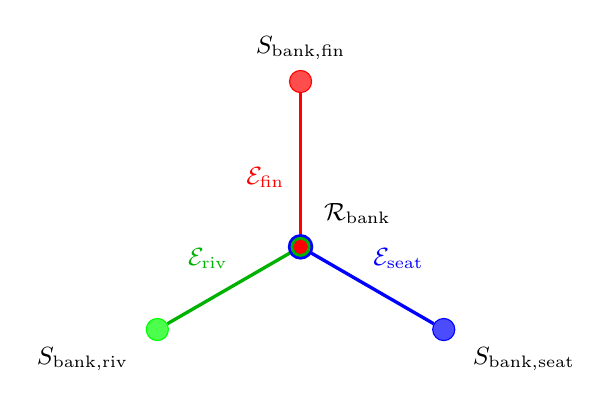
\begin{tikzpicture}[scale=0.5,
    outer/.style={circle, draw, minimum size=8pt,
                  inner sep=0pt, font=\footnotesize},
    lab/.style={font=\small}]
% central shared reference-subspace vertex
\coordinate (c) at (0,0);

\node[lab, above right=7pt] at (c)
{$\mathcal R_{\rm bank}$};

% outer sense-subspace vertices
\node[outer, red, fill=red!70,
      label={[lab]above:
      $S_{{\rm bank},{\rm fin}}$}]
      (fin) at (90:4.2cm) {};

\node[outer, green, fill=green!70,
      label={[lab, xshift=-4pt]below left:
      $S_{{\rm bank},{\rm riv}}$}]
      (riv) at (210:4.2cm) {};

\node[outer, blue, fill=blue!70,
      label={[lab, xshift=4pt]below right:
      $S_{{\rm bank},{\rm seat}}$}]
      (seat) at (330:4.2cm) {};

% hyperedges labelled by context
\draw[very thick, red] (c) --
      node[lab, left=2pt, pos=0.45]
      {$\mathcal E_{\rm fin}$} (fin);

\draw[very thick, green!70!black] (c) --
      node[lab, above left=1pt, pos=0.45]
      {$\mathcal E_{\rm riv}$} (riv);

\draw[very thick, blue] (c) --
      node[lab, above right=1pt, pos=0.45]
      {$\mathcal E_{\rm seat}$} (seat);

% central concentric disks
\filldraw[blue, very thick] (c) circle (8pt);
\filldraw[green!70!black, very thick] (c) circle (6pt);
\filldraw[red, very thick] (c) circle (4pt);
\end{tikzpicture}
\caption{%
Incidence schematic for the polysemous token ``bank,'' retaining the original
star geometry.  The center is the shared reference subspace
$\mathcal R_{\rm bank}$ and the outer nodes are the financial, river-edge,
and seat/bench sense subspaces in $\mathcal R_{\rm bank}^{\perp}$.  Each
colored spoke $\mathcal E_C$ labels a context incidence associated with
$\Pi_{{\rm bank},C}$; it is not a vector, map, or causal arrow.  In a complete
contextuality hypergraph, additional outcome sectors would complete each
measurement context.  The aircraft-banking sense could be added as a fourth
spoke but is omitted for clarity.
}
\label{fig:reference-subspace}
\end{figure}

\subsection{Relation to dynamic contextual embeddings}
\label{sec:dynamic}

Transformers already handle polysemy dynamically. The hidden state
$h_\ell(t\mid x)$ of token $t$ at layer $\ell$ depends on context $x$.
The reference-subspace and shared-sector operator hypotheses are not
alternative hardware architectures; they are proposed organizations and
readouts of these observed trajectories.

Given a candidate reference subspace $\mathcal R_t$ and its projector $P_t$,
write
%
\begin{align}
\label{eq:layer-decomp}
h_\ell(t\mid x)
&=P_t h_\ell(t\mid x)+z_\ell(t,x),\\
z_\ell(t,x)&=(I-P_t)h_\ell(t\mid x)
\in\mathcal R_t^\perp.\nonumber
\end{align}
%
The decomposition is automatic; the hypothesis is not. It predicts that
$P_t h_\ell(t\mid x)$ tracks token identity or engagement, while
$z_\ell(t,x)$ carries most sense-disambiguating information. Sense labels
should be more separable in $\mathcal R_t^\perp$ than in the orthogonal
complements of matched control subspaces. For each sense $C$, the projected
states $z_\ell(t,x)$ should also concentrate near the low-dimensional
subspace $S_{t,C}\subset\mathcal R_t^\perp$.

Thus the critical question is not whether contextual embeddings move; they
do. It is whether their sense-relevant movement has a privileged organization
relative to a token-associated reference subspace, and whether conditional
application of $\Pi_{t,C}$ explains that movement better than matched
unstructured projectors.

% ======================================================================
\section{Attention and latent context selection}
\label{sec:attention}
% ======================================================================

A standard attention head computes
%
\begin{equation}
\label{eq:attention}
h'=\sum_j\alpha_j\nu_j,
\qquad
\alpha_j=
\frac{\exp(q_{\rm att}\T k_{{\rm att},j}/\sqrt{d_{\rm head}})}
{\sum_{j'}\exp(q_{\rm att}\T k_{{\rm att},j'}/\sqrt{d_{\rm head}})} .
\end{equation}
%
$q_{\rm att},k_{{\rm att},j}\in\R^{d_{\rm head}}$ are the query and key
vectors of that head.  The local head width $d_{\rm head}$ is an architectural
quantity, not necessarily the selected carrier dimension $d$ used in the
geometric null model.
Keys and values are produced by different learned maps, so value vectors
are not generally coefficients of a dual basis for the key vectors.
Attention is therefore not literal basis reconstruction.

The useful analogy is softer. Attention routes information: it amplifies
some contextual directions and suppresses others. In the terminology of
Sec.~\ref{sec:reference}, this resembles context-dependent subspace
selection. A literal basis-reconstruction interpretation would require
additional constraints, such as approximately Parseval keys and values
implementing the corresponding dual reconstruction. We do not assume this.

A usable context selector cannot receive the true sense label at inference.
Let a learned router $r_\theta(x,t)$ depend only on the available sequence and
token state, and define
%
\begin{equation}
\label{eq:context-temp}
p_\theta(C\mid x,t)=
\frac{\exp(r_{\theta,C}(x,t)/T)}
{\sum_{C'}\exp(r_{\theta,C'}(x,t)/T)} .
\end{equation}
%
The router may use the illustrative score in Eq.~\eqref{eq:sense-score}, but
need not do so.  Its weights provide a soft shared-sector projection:
%
\begin{equation}
\label{eq:soft-observable-embedding}
\begin{aligned}
\bar h_t(x)
&=\sum_C p_\theta(C\mid x,t)\,h_{t,C}(x)\\
&=\sum_C p_\theta(C\mid x,t)\,\Pi_{t,C}h(x).
\end{aligned}
\end{equation}
%
Hard selection uses the largest router probability; soft selection uses
Eq.~\eqref{eq:soft-observable-embedding}.  This is an ordinary
mixture-of-projectors computation.  Attention may supply its routing signal,
but neither the shared sector nor the operator structure follows from standard
attention.  The constrained model must therefore be compared with
parameter-matched mixture-of-experts and unstructured low-rank alternatives.

% ======================================================================
\section{Discussion}
\label{sec:discussion}
% ======================================================================

The mathematical ingredients of the geometric analysis are standard
coherence, concentration, and fixed-target readout estimates.  Their role is
not to turn the condition $\Nsem>d$ into a discovery, but to provide calibrated
null predictions for an empirically extracted dictionary.  The discriminating
question is whether training systematically redistributes overlap: frequently
coactive features should incur less interference, and held-out readout should
improve relative to isotropic and activity-matched controls.

The shared-sector operator proposal is logically independent of that null
model.  It asserts that trajectories of some polysemous tokens admit a
specific constrained organization.  Neither a fitted common subspace nor a
nonzero commutator is sufficient evidence.  Evidence requires generalization
to held-out contexts and an advantage over equally expressive unstructured
projectors or mixture models.

\subsection{Relation to superposition and sparse autoencoders}
\label{sec:superposition}

The superposition hypothesis holds that neural networks may represent more
features than they have neurons by using nonorthogonal directions with sparse
activity~\cite{elhage2022superposition,bricken2023monosemanticity}.  The null
model separates dictionary coexistence from simultaneous linear readout.  In
the isotropic, weak-dependence model, many directions can coexist while a
fixed-target correlation decoder accumulates interference of scale
$\sqrt{k/d}$.  Sparse activity controls that interference for this decoder;
it is not asserted to be universally necessary for structured dictionaries or
nonlinear recovery.

Sparse autoencoders (SAEs) give a concrete empirical interface. They
approximate layer activations as sparse expansions over learned decoder
directions, making the $w_i$ of Eq.~\eqref{eq:hidden} measurable
objects rather than hypothetical features. Recent work has scaled SAEs,
studied SAE feature geometry, and automated interpretation of large
numbers of latents~\cite{gao2025scaling,li2025geometry,paulo2025automatically,shu2025survey}. In the
present framework, SAE decoder directions make the null calibration and
coactivation-weighted diagnostic measurable, while sense-conditioned SAE
activation clusters can test the stronger reference-subspace hypothesis.

\subsection{A coactivation-weighted interference diagnostic}
\label{sec:coactivation-diagnostic}

The active-set size $k$ is a crude summary because it ignores which features
appear together.  For the fixed-target correlation readout, define an ordered
nonnegative pair weight
%
\begin{equation}
\label{eq:coactivation}
c_{ij}:=\Prob(i,j\text{ active})
\E[x_j^2\mid i,j\text{ active}]\,\omega_i,
\end{equation}
%
where $\omega_i$ records the task importance of accurately reading feature
$i$.  Under the same zero-mean or weak-correlation assumptions used for the
RMS calculation, a natural held-out diagnostic is
%
\begin{equation}
\label{eq:int-energy}
\Eint=
\sum_{i\neq j}
c_{ij}(w_i\T w_j)^2 .
\end{equation}
%
Unlike maximum coherence, Eq.~\eqref{eq:int-energy} does not penalize a large
overlap merely because it exists.  If training or selection penalizes readout
error, it predicts pressure toward smaller overlaps specifically for important
features that coactivate.  Mutually exclusive features can share geometric
resources at much lower cost.  This conditional redistribution, assessed
against controls matched for marginal activity, amplitudes, feature
importance, and dictionary size, is the paper's substantive geometric
prediction.

\subsection{Limitations}
\label{sec:limitations}

The framework can fail in several ways.

First, the deterministic Welch bound constrains the coherence of a specified
$N$-vector dictionary, but the crowding expression in
Eq.~\eqref{eq:max-overlap} assumes independent isotropic directions.  It is a
typical null scale, not an optimal-code upper bound or a semantic impossibility
theorem.  The inequality $N>d$ is only the inclusion criterion for the
overcomplete regime studied here; no lower usefulness boundary occurs at
$N=d$.

Second, the nominal layer width need not equal the selected carrier rank $d$.
Contextual embeddings can be anisotropic, and the occupied carrier can vary
strongly by layer and training regime
\cite{ethayarajh2019,gao2019representation,mu2018allbutthetop,razzhigaev2024shape}. Whitening and
related postprocessing can partially restore isotropic geometry
\cite{gao2019representation,mu2018allbutthetop,su2021whitening}. At the same time, anisotropy should not
be treated as an automatic or universal property of all Transformer
representations~\cite{machina2024anisotropy}. The rule used to select or
whiten a $d$-dimensional carrier must therefore be reported. Whitening also
changes the metric in which overlaps are measured, and the covariance spectrum
may contain information not summarized by one rank. We do not introduce a
second dimension symbol, but $d$ is protocol-dependent rather than an
intrinsic semantic constant.

Third, $N$ depends on the feature-extraction, normalization, and
duplicate-removal rules.  A claimed departure from the null may instead expose
a poor dictionary, dependence among samples, finite-size effects, or a changed
metric.  These alternatives must be checked before attributing the departure
to learned semantic organization.

Fourth, the reference-subspace pattern may simply be descriptively wrong.
Trained models may represent polysemy without a preferred token-associated
direction or subspace.  A low-rank fit found after inspecting test labels is
not evidence; ranks, candidate references, and routers must be selected on
training data and evaluated out of sample.

Fifth, the law $\sint\sim\sqrt{k/d}$ concerns a fixed-target correlation
readout with random-like directions and weakly correlated signs or amplitudes.
It is neither a joint sparse-recovery theorem nor a universal equality.
Structured dictionaries, nonlinear decoders, multiple comparisons over
inactive features, and correlated errors can change the scaling.

Finally, the operator model has choices: the candidate reference subspace
$\mathcal R_t$, the router, the local ranks, and any spectra in
Eq.~\eqref{eq:context-observable}.  The true sense label cannot be supplied to
the router at test time.  Eigenvalues are not identified by subspaces alone,
and a fitted nonzero commutator is generic.  These choices add evidence only
through held-out prediction, compression, or prespecified order effects.

\subsection{Empirical predictions}
\label{sec:predictions}

The key empirical task is to distinguish a null calibration from three
substantive hypotheses.

\emph{Null calibration (not a semantic claim).}
For a dictionary independently established to be overcomplete, compare its
coherence, overlap distribution, and fixed-target readout error with isotropic
and activity-matched controls.  Agreement with Eq.~\eqref{eq:max-overlap} is a
baseline result, not evidence that overcompleteness is useful; departure from
it must be diagnosed before being called learned structure.

{Claim A: privileged token reference subspace.}
For a polysemous token $t$, there exists a privileged token-associated
subspace $\mathcal R_t$ such that sense-relevant variation is better
exposed in $\mathcal R_t^\perp$ than in the orthogonal complements of
matched control subspaces of the same dimension.

{Claim B: low-dimensional sense subspaces.}
Within $\mathcal R_t^\perp$, sense-conditioned states admit a cross-validated
low-rank description that predicts or compresses held-out states better than
shuffled-label, ordinary clustering, and matched-subspace controls.  Related
polysemous senses need not have minimal cross-sense coherence.

{Claim C: shared-sector context operators.}
A non-oracular router and context projectors $\Pi_{t,C}$ sharing $P_t$ improve
held-out contextual prediction or compression relative to parameter-matched
unstructured projectors and mixture-of-experts models.  A commutator matters
only if it predicts order effects defined independently of the fitted
operators.

These claims can fail independently.  The null calibration can hold while all
three structural claims fail.  Claim A can hold while sense information
remains high-dimensional.  Claim B can hold relative to a non-token-associated
subspace, in which case Claim A fails.  Claims A and B can hold even if the
operator constraint in Claim C adds no predictive value.

The following tests separate the possibilities.

\begin{enumerate}
\item \emph{Null-model calibration.}
Fix the carrier metric, spectral threshold or whitening rule, feature extractor,
and duplicate criterion before evaluation.  Report the selected rank $d$,
dictionary size $N$, maximum coherence, the full overlap distribution, and
active-set statistics.  Compare with the Welch floor, isotropic dictionaries,
and controls matched for marginal activity and coactivation.  Treat
Eq.~\eqref{eq:max-overlap} as a finite-sample null prediction, not a pass/fail
capacity test.

\item \emph{Reference-subspace test.}
For a polysemous token, choose candidate reference subspaces generated
by the normalized static input embedding, mean contextual embedding,
learned token-specific directions, or a low-dimensional combination of
these. Project layer states as in Eq.~\eqref{eq:layer-decomp}. Sense labels
should be better separated in $\mathcal R_t^\perp$ than in orthogonal
complements obtained after ordinary centering, token-mean subtraction,
top-principal-component removal, and random, frequency-matched, or
layer-matched control subspaces of the same rank.  Compare held-out
classification, compression, or incremental mutual information, with
permutation over sense labels and bootstrap over token instances.

\item \emph{Operational subspace test.}
For each sense $s$, collect projected states
$z_\ell(t,x)\in\mathcal R_t^\perp$ and estimate a low-rank subspace by PCA or
probabilistic factor analysis. Select $q_s$ without test-label leakage and use
an orthonormal basis $B_{t,s}$.  Evaluate held-out reconstruction and sense
prediction against shuffled labels, ordinary supervised subspaces, and
unsupervised clustering of equal rank.  Report
$\opnorm{B_{t,s}\T B_{t,s'}}$ descriptively, without assuming related senses
must be nearly orthogonal.

\item \emph{Gated-readout test.}
Linear probes trained on $z_\ell(t,x)$ should perform comparably to
probes trained on the full state $h_\ell(t\mid x)$, while probes
restricted to the reference component $P_t h_\ell(t\mid x)$ should provide
less incremental sense information after frequency, syntax, and sense-prior
controls.  Near-chance performance is not required because the reference
component may legitimately retain correlated information.

\item \emph{Shared-sector operator test.}
Fit $P_t$, $B_{t,C}$, and the router on training contexts, then evaluate
Eq.~\eqref{eq:soft-observable-embedding} without true sense labels on held-out
instances. Compare with unconstrained low-rank projectors, ordinary contextual
probes, parameter-matched mixture-of-experts models, and shuffled context
labels.  If an order claim is made, define the sequential linguistic or model
intervention independently; then ask whether
$\opnorm{[\Pi_{t,C},\Pi_{t,C'}]}$ predicts the measured asymmetry.  Merely
obtaining a nonzero commutator does not pass the test.

\item \emph{Isotropic-null overlap test.}
Independent isotropic directions have signed inner-product variance $1/d$.
Compare the full pairwise distribution of token embeddings or SAE decoder
directions with that null after the carrier and metric have been selected.
Deviations may reflect dependence, anisotropy, extraction choices, or learned
alignment; quasi-orthogonality alone does not predict variance $1/d$.

\item \emph{Synthetic concurrency degradation.}
At a fixed layer, inject controlled superpositions
%
\begin{equation}
h_k=h_0+\lambda\sum_{j=1}^k x_j w_j,
\end{equation}
%
using directions $w_j$ obtained independently, for example from SAE
decoder directions or frozen linear probes. As $k$ increases, readout
should degrade smoothly on the scale $\sqrt{k/d}$ for random-like
directions under the specified correlation decoder.  Include norm-preserving,
random-direction, activation-frequency, and out-of-distribution controls;
degradation by itself does not validate semantic superposition.

\item \emph{Coactivation-dependent geometry.}
At matched marginal activation frequency, feature similarity, SAE
reconstruction error, amplitude, and task relevance, important frequently
coactive features should contribute less to Eq.~\eqref{eq:int-energy} than
activity-matched controls.  This tests learned redistribution of interference,
independently of the reference-subspace hypothesis.
\end{enumerate}

\subsection{Scope of the quantum analogy}
\label{sec:quantum}

The analogy to quantum contextuality is structural and limited. Both settings
can describe alternatives by observables with context-dependent eigenspaces.
In the proposed construction, several contexts share the spectral projector
$P_t$ while differing on complementary sense sectors.  We call this
``intertwined'' only in the explicitly declared contextuality-inspired
incidence sense, not in the standard operator-theoretic sense.  The shared
$P_t$ cancels from the commutator, so it is the relative geometry of the sense
sectors that may produce order dependence.  Figure~\ref{fig:reference-subspace}
records the displayed incidence pattern; omitted complementary outcome sectors
would be required to complete each measurement context in a full contextuality
hypergraph.  Equations~\eqref{eq:context-projector}--
\eqref{eq:context-observable} provide the corresponding operator
parameterization.  Vectors, subspaces, projectors, and observables are distinct
mathematical types.

Quantum contextuality has the force of no-go theorems such as
Kochen--Specker~\cite{specker-60,kochen1}; no analogous theorem is claimed
here for semantic embeddings.  Real symmetric matrices can be noncommuting
while still being stored and evaluated on an ordinary classical computer, and
generic fitted projectors are commonly noncommuting.  Thus noncommutativity by
itself supplies neither a semantic result, Born probabilities, nor physical
quantumness.

Three levels of analysis should not be conflated.
%
\begin{enumerate}
\item \emph{Classical high-dimensional representation.}
A present-day Transformer carries real-valued hidden states through
attention, nonlinear feed-forward maps, residual connections, and
normalization.  Concentration, quasi-orthogonality, feature superposition,
dynamic embeddings, and finite readout are all available at this level.
None requires quantum probability or quantum hardware.

\item \emph{Quantum-like semantic or contextual formalism.}
States, contexts, bases, interference terms, noncommuting questions, or
measurement-like updates may be used as an abstract model of meaning even
when the implementation remains classical.  The relevant issue is not the
vocabulary but whether this extra structure improves compression,
explanation, or prediction relative to an ordinary contextual embedding
model.

\item \emph{Genuine quantum machine learning or quantum attention.}
Here semantic states would be encoded in qubits or other physical quantum
degrees of freedom, intermediate evolution would be unitary, phase would
affect interference, and measurement would follow quantum probability.  A
standard Transformer does none of these things.
\end{enumerate}
%

The random-dictionary and linear-readout baselines belong entirely to the first
level.  Shared-sector projection is also an ordinary classical computation.
The proposal earns the stronger quantum-like interpretation only if its
operator constraints or prespecified order effects improve prediction,
compression, or explanation relative to equally expressive classical
baselines.  Even a positive result would support a useful formalism, not
physical quantum computation; phase-sensitive dynamics and Born-rule
measurement remain absent.

The dimension of $\mathcal R_t$ is also explicit. In Hilbert-space quantum
logic, different contexts can share one observable, as in the familiar
tripod-like case, or several observables; a four-dimensional example has
two contexts with two common observables~\cite{svozil:040102}. The semantic
analogue is $\dim(\mathcal R_t)=p$: $p=1$ is the simplest case, while
$p>1$ permits several token-associated reference directions. In every case,
sense-specific information is hypothesized to occupy subspaces of
$\mathcal R_t^\perp$.

% ======================================================================
\section{Conclusion}
\label{sec:conclusion}
% ======================================================================

This chapter treats overcompleteness as an empirical starting condition, not
as a theorem.  After fixing a carrier, metric, and feature-extraction rule, the
dictionary under study has size $N>d$ in a carrier of rank $d$.  The classical
geometry then supplies calibrated baselines.  The Welch bound is a genuine
deterministic coherence floor for a specified $N$ and $d$.  By contrast, an
isotropic random dictionary predicts a worst overlap of order
$2\sqrt{\log N/d}$, and a random-like active set produces fixed-target linear
readout interference of order $\sqrt{k/d}$.  The associated scale
$\exp(d\varepsilon^2/4)$ is a random-code crowding crossover, not a universal
upper bound and not evidence that $N\le d$ is semantically deficient.

The more consequential geometric hypothesis concerns where overlap is placed.
Important features that frequently coactivate should contribute less
coactivation-weighted interference than activity-, amplitude-, and
importance-matched controls, whereas mutually exclusive features may share
representational resources at lower cost.  This turns standard geometry into
a falsifiable claim about learned organization rather than a restatement of
finite-dimensional linear algebra.

The second proposal is a constrained operator model of polysemy.  Context
projectors share a token-associated invariant sector and differ on
low-dimensional sense subspaces in its orthogonal complement.  Conditional
projection yields a context-specific embedding, and a learned non-oracular
router supplies hard or soft context selection.  The common projector does not
cause noncommutativity, and a nonzero fitted commutator has no evidential force
by itself.  The model succeeds only if the shared-sector constraint improves
held-out prediction or compression over parameter-matched unstructured models,
or if its commutators predict independently specified order effects.

The null-model calibration and the shared-sector hypothesis can fail
independently.  A trained dictionary may redistribute interference without a
privileged token reference subspace; conversely, a useful shared-sector model
could exist even when global feature geometry is poorly described by an
isotropic code.  Keeping these claims separate preserves an informative
outcome in either case.

The construction is quantum-inspired, not a claim that a Transformer is a
quantum device.  It uses real matrices on classical hardware and introduces no
Born rule, unitary dynamics, or physical measurement.  Quantum terminology is
earned only insofar as the constrained operator structure provides additional,
held-out explanatory or predictive value.

\begin{acknowledgments}
OpenAI Codex (GPT-5) was used to assist with literature organization, \LaTeX{}
editing, and checks of derivations.  The authors specified the scientific
direction and prompts; model output retained in the manuscript was checked
against the cited sources and explicit calculations.  The authors accept full
responsibility for the final text.

This research was funded in part by the Austrian
Science Fund (FWF), Grant digital object identifier (DOI)
\href{https://doi.org/10.55776/PIN5424624}{10.55776/PIN5424624}.
The author acknowledges FWF and TU Wien Bibliothek for financial support through its
Open Access Funding Programme.

The authors declare no conflict of interest.
\end{acknowledgments}

\bibliography{svozil}

\end{document}
